\documentclass[journal,12pt,twocolumn]{IEEEtran}
%
\usepackage{setspace}
\usepackage{gensymb}
%\doublespacing
\singlespacing

\usepackage{graphicx}
\usepackage[cmex10]{amsmath}
\usepackage{amsmath,amsthm}
\usepackage{mathrsfs}
\usepackage{txfonts}
\usepackage{stfloats}
\usepackage{bm}
\usepackage{cite}
\usepackage{cases}
\usepackage{subfig}

\usepackage{longtable}
\usepackage{multirow}
\usepackage{commath}
\usepackage{enumitem}
\usepackage{mathtools}
\usepackage{steinmetz}
\usepackage{tikz}
\usepackage{circuitikz}
\usepackage{verbatim}
\usepackage{tfrupee}
\usepackage[breaklinks=true]{hyperref}

\usepackage{tkz-euclide}

\usetikzlibrary{calc,math}
\usepackage{listings}
\usepackage{color}                                            
\usepackage{array}                                            
\usepackage{longtable}                                        
\usepackage{calc}                                             
\usepackage{multirow}                                         
\usepackage{hhline}                                           
\usepackage{ifthen}                                           
\usepackage{lscape}     
\usepackage{multicol}
\usepackage{chngcntr}

\DeclareMathOperator*{\Res}{Res}

\renewcommand\thesection{\arabic{section}}
\renewcommand\thesubsection{\thesection.\arabic{subsection}}
\renewcommand\thesubsubsection{\thesubsection.\arabic{subsubsection}}

\renewcommand\thesectiondis{\arabic{section}}
\renewcommand\thesubsectiondis{\thesectiondis.\arabic{subsection}}
\renewcommand\thesubsubsectiondis{\thesubsectiondis.\arabic{subsubsection}}

\hyphenation{op-tical net-works semi-conduc-tor}
\def\inputGnumericTable{}                                 

\lstset{
	%language=C,
	frame=single, 
	breaklines=true,
	columns=fullflexible
}
\lstset{
	%language=TeX,
	frame=single, 
	breaklines=true
}

\begin{document}
	
	
	\newtheorem{theorem}{Theorem}[section]
	\newtheorem{problem}{Problem}
	\newtheorem{proposition}{Proposition}[section]
	\newtheorem{lemma}{Lemma}[section]
	\newtheorem{corollary}[theorem]{Corollary}
	\newtheorem{example}{Example}[section]
	\newtheorem{definition}[problem]{Definition}
	
	\newcommand{\BEQA}{\begin{eqnarray}}
		\newcommand{\EEQA}{\end{eqnarray}}
	\newcommand{\define}{\stackrel{\triangle}{=}}
	\bibliographystyle{IEEEtran}
	\providecommand{\mbf}{\mathbf}
	\providecommand{\pr}[1]{\ensuremath{\Pr\left(#1\right)}}
	\providecommand{\qfunc}[1]{\ensuremath{Q\left(#1\right)}}
	\providecommand{\sbrak}[1]{\ensuremath{{}\left[#1\right]}}
	\providecommand{\lsbrak}[1]{\ensuremath{{}\left[#1\right.}}
	\providecommand{\rsbrak}[1]{\ensuremath{{}\left.#1\right]}}
	\providecommand{\brak}[1]{\ensuremath{\left(#1\right)}}
	\providecommand{\lbrak}[1]{\ensuremath{\left(#1\right.}}
	\providecommand{\rbrak}[1]{\ensuremath{\left.#1\right)}}
	\providecommand{\cbrak}[1]{\ensuremath{\left\{#1\right\}}}
	\providecommand{\lcbrak}[1]{\ensuremath{\left\{#1\right.}}
	\providecommand{\rcbrak}[1]{\ensuremath{\left.#1\right\}}}
	\theoremstyle{remark}
	\newtheorem{rem}{Remark}
	\newcommand{\sgn}{\mathop{\mathrm{sgn}}}
	\providecommand{\abs}[1]{\(\left\vert#1\right\vert\)}
	\providecommand{\res}[1]{\Res\displaylimits_{#1}} 
	\providecommand{\norm}[1]{\(\left\lVert#1\right\rVert\)}
	%\providecommand{\norm}[1]{\lVert#1\rVert}
	\providecommand{\mtx}[1]{\mathbf{#1}}
	\providecommand{\mean}[1]{E\(\left[ #1 \right]\)}
	\providecommand{\fourier}{\overset{\mathcal{F}}{ \rightleftharpoons}}
	%\providecommand{\hilbert}{\overset{\mathcal{H}}{ \rightleftharpoons}}
	\providecommand{\system}{\overset{\mathcal{H}}{ \longleftrightarrow}}
	%\newcommand{\solution}[2]{\textbf{Solution:}{#1}}
	\newcommand{\solution}{\noindent \textbf{Solution: }}
	\newcommand{\cosec}{\,\text{cosec}\,}
	\providecommand{\dec}[2]{\ensuremath{\overset{#1}{\underset{#2}{\gtrless}}}}
	\newcommand{\myvec}[1]{\ensuremath{\begin{psmallmatrix}#1\end{psmallmatrix}}}
	\newcommand{\mydet}[1]{\ensuremath{\begin{vmatrix}#1\end{vmatrix}}}
	%\numberwithin{equation}{section}
	\numberwithin{equation}{subsection}
	%\numberwithin{problem}{section}
	%\numberwithin{definition}{section}
	\makeatletter
	\@addtoreset{figure}{problem}
	\makeatother
	\let\StandardTheFigure\thefigure
	\let\vec\mathbf
	%\renewcommand{\thefigure}{\theproblem.\arabic{figure}}
	\renewcommand{\thefigure}{\theproblem}
	%\setlist[enumerate,1]{before=\renewcommand\theequation{\theenumi.\arabic{equation}}
	%\counterwithin{equation}{enumi}
	%\renewcommand{\theequation}{\arabic{subsection}.\arabic{equation}}
	\def\putbox#1#2#3{\makebox[0in][l]{\makebox[#1][l]{}\raisebox{\baselineskip}[0in][0in]{\raisebox{#2}[0in][0in]{#3}}}}
	\def\rightbox#1{\makebox[0in][r]{#1}}
	\def\centbox#1{\makebox[0in]{#1}}
	\def\topbox#1{\raisebox{-\baselineskip}[0in][0in]{#1}}
	\def\midbox#1{\raisebox{-0.5\baselineskip}[0in][0in]{#1}}
	\vspace{3cm}
	\title{Assignment 3}
	\author{Addagalla Satyanarayana}
	\maketitle
	\newpage
	%\tableofcontents
	\bigskip
	\renewcommand{\thefigure}{\theenumi}
	\renewcommand{\thetable}{\theenumi}
\begin{abstract}
This document uses the properties of a parallelogram to prove a statement
\end{abstract}
Download latex-tikz codes from 
%
\begin{lstlisting}
https://github.com/AddagallaSatyanarayana/AI5006/tree/master/Assignment3/assignment3.tex
\end{lstlisting}
%
\section{Problem}
	Prove that the sum of the squares of diagonals of parallelogram is equal to the sum of the squares of its sides.


\section{Explanation}
Given a parallelogram ABCD we have to prove that
\begin{figure}[!ht]
	\centering
	\resizebox{\columnwidth}{!}{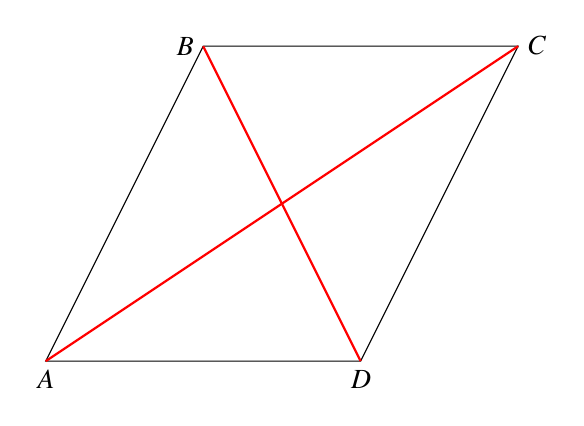
\begin{tikzpicture}	
	\draw (0,0) node[anchor=north]{$A$}
	-- (2,4) node[anchor=east]{$B$}
	-- (6,4) node[anchor=west]{$C$}
	-- (4,0) node[anchor=north]{$D$}
	-- cycle;
	\draw[red][thick] (2,4) -- (4,0) 	-- cycle;
	\draw[red][thick] (6,4) -- (0,0) 	-- cycle;
\end{tikzpicture}}
	\caption{parallelogram ${ABCD}$}
	\label{fig1:Parallelogram}
\end{figure}
	
\begin{multline}
	\norm{\vec{A-C}}^2 + \norm{\vec{B-D}}^2 =\\ \norm{\vec{A-B}}^2+\norm{\vec{B-C}}^2+\norm{\vec{D-C}}^2+\norm{\vec{A-D}}^2\label{eq:1}
\end{multline}

\section{Solution}
 The diagonals of  parallelogram are
\begin{align}
	\vec{A-C} = (\vec{A-D}) +(\vec{D-C})\\
	\vec{B-D} = (\vec{A-D}) -(\vec{A-B})
\end{align} 
The sum  of the squares of diagonals is
\begin{multline}
	\norm{\vec{A-C}}^2 +\norm{\vec{B-D}}^2 =\\ \norm{(\vec{A-D}) +(\vec{D-C})}^2+ \norm{(\vec{A-D}) -(\vec{A-B})}^2
\end{multline}
\begin{multline}
	\norm{\vec{A-C}}^2 +\norm{\vec{B-D}}^2 = \\\norm{\vec{A-D}}^2 +\norm{\vec{D-C}}^2 + 2{(\vec{A-D})}^T{(\vec{D-C})}+\\\norm{\vec{A-D}}^2+\norm{\vec{A-B}}^2-2{(\vec{A-D})}^T{(\vec{A-B})}\label{eq:2}
\end{multline}
\begin{multline}
	\norm{\vec{A-C}}^2 +\norm{\vec{B-D}}^2 = \\\norm{\vec{A-D}}^2 +\norm{\vec{D-C}}^2 + 2\norm{\vec{A-D}}\norm{\vec{D-C}}\cos(180\degree-\angle{ADC})+\\ \norm{\vec{A-D}}^2+\norm{\vec{A-B}}^2-2 {\norm{\vec{A-D}}\norm{\vec{A-B}}}\cos\angle{DAB}\label{eq:3}
\end{multline}

In the parallelogram $ABCD$  
\begin{align}
	\norm{\vec{A-D}}&=\norm{\vec{B-C}}\label{eq:4}\\
	\norm{\vec{A-B}} &= \norm{\vec{D-C}}\label{eq:5}\\
	\angle{ADC} + \angle{DAB} &= 180\degree\\
	\angle{DAB} &= 180\degree -\angle{ADC} \label{eq:6}
\end{align}
From equation \eqref{eq:3},\eqref{eq:4},\eqref{eq:5}  and \eqref{eq:6}
\begin{multline}
	\norm{\vec{A-C}}^2 +\norm{\vec{B-D}}^2 = \\\norm{\vec{B-C}}^2 +\norm{\vec{D-C}}^2 + 2\norm{\vec{A-D}}\norm{\vec{A-B}}\cos\angle{DAB}+\\ \norm{\vec{A-D}}^2+\norm{\vec{A-B}}^2-2{\norm{\vec{A-D}}\norm{\vec{A-B}}}\cos\angle{DAB}\label{eq:7}
\end{multline}
Simplifying equation \eqref{eq:7}
\begin{multline}
	\norm{\vec{A-C}}^2 + \norm{\vec{B-D}}^2 =\\ \norm{\vec{A-B}}^2+\norm{\vec{B-C}}^2+\norm{\vec{D-C}}^2+\norm{\vec{A-D}}^2\label{eq:8}
\end{multline}
The equations \eqref{eq:1}  and \eqref{eq:8} are equal,hence proved
\end{document}